\documentclass[11pt]{article}
\usepackage{amsmath, color, graphicx, indentfirst, float, wrapfig}
\usepackage[margin=1in]{geometry}

\title{Computational Physics: Homework 1 }
\author{Austin McDowell}
 
\begin{document}
\maketitle

\section*{Problem 1}
\subsection*{Introduction}
In this problem we created a plot of the Mandelbrot set. The Mandelbrot set created iteratively using the equation
\begin{equation}
\label{eq:man_eq}
z^\prime = z^2 + c
\end{equation}
where $z$ is a complex input number and $c = x + iy$ is another complex number used to create the output, $z^\prime$. For a pair of $x$ and $y$ values we create the complex number $c$ and start with $z=0$. We then iterate using equation (\ref{eq:man_eq}) and if $|z|>2$ then the point at $(x,y)$ is \textbf{not} in the Mandelbrot set. 

\subsection*{Methods}
For our purposes we made a evenly spaced grid in $x$ and $y$ ranging from -2 to 2 with which the values for $c$ were made. For each point, we iterated a maximum of 100 times to check if the point at $(x,y)$ was in the set. At first our grid size was 100x100 but it was ultimately increased to 750x750 to produce the final plots.

To keep track of whether an $(x,y)$ pair was in the set, an array of zeros, $Z$, of size $(N,N)$ was created where $N$ is the size of the $x$ and $y$ grids. If, $|z|$ was ever greater than 2, the corresponding point in $Z$ was left as 0. If, after 100 iterations, the value for $|z|$ was less than 2, the corresponding point was given a value of 1. This method was used to make a 'binary' Mandelbrot set where points are considered either 'in' or 'out'. Additionally, a Mandelbrot 'density' plot was made where the value in $Z$ was incremented based on the number of iterations before $|z|$ becomes larger than 2. 

\subsection*{Results}
\begin{figure}[H]
  \centering
  \begin{minipage}[t]{0.5\textwidth}
    \centering
    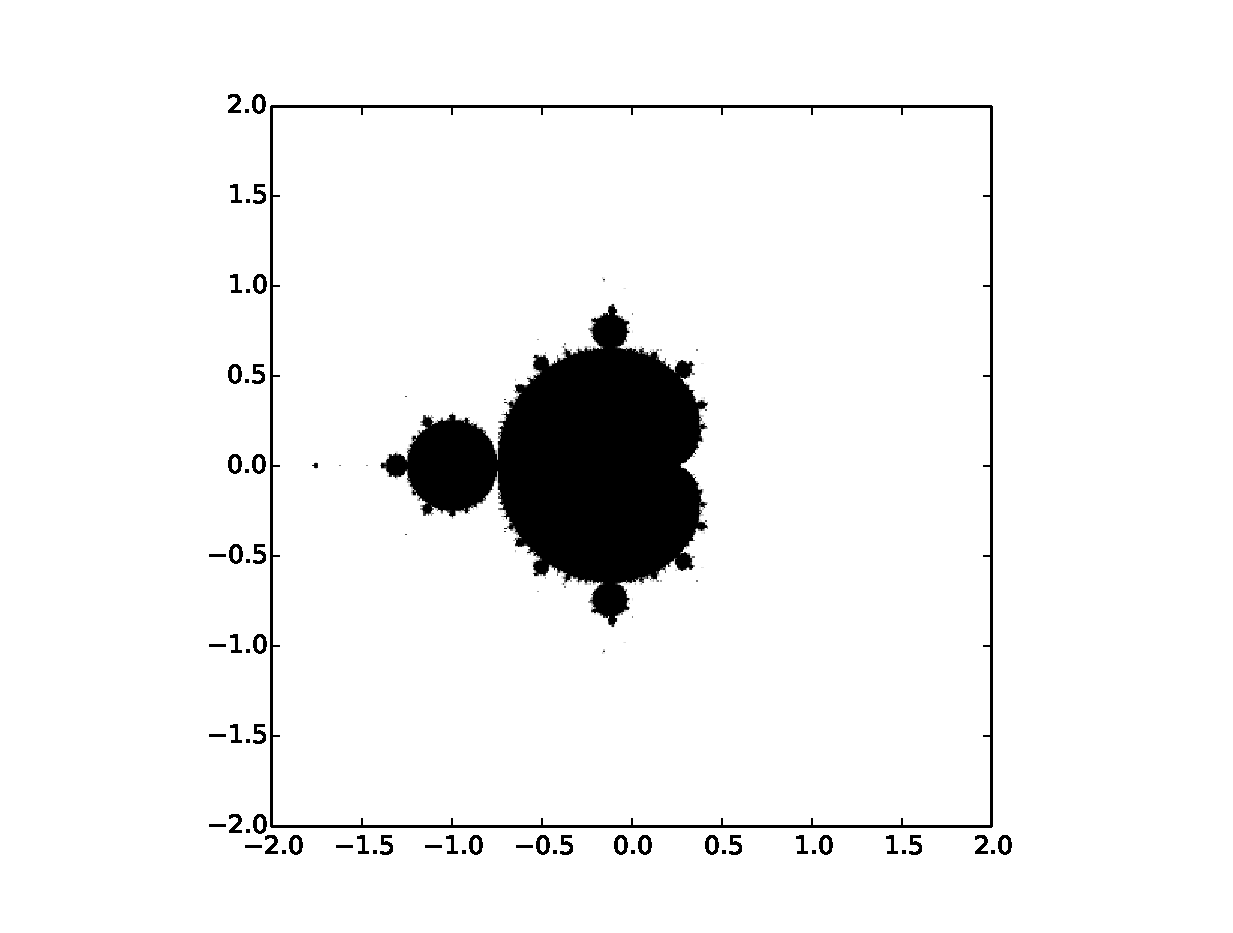
\includegraphics[width=\linewidth]{mandel_1.eps}
    \caption{\scriptsize 'Binary' Mandelbrot image. The black region contains the points where $|z|<2$}
    \label{fig:elevels}
   \end{minipage}
\end{figure}

\begin{figure}[H]
  \centering
  \begin{minipage}[t]{0.4\textwidth}
    \centering
    \vspace{0pt}
    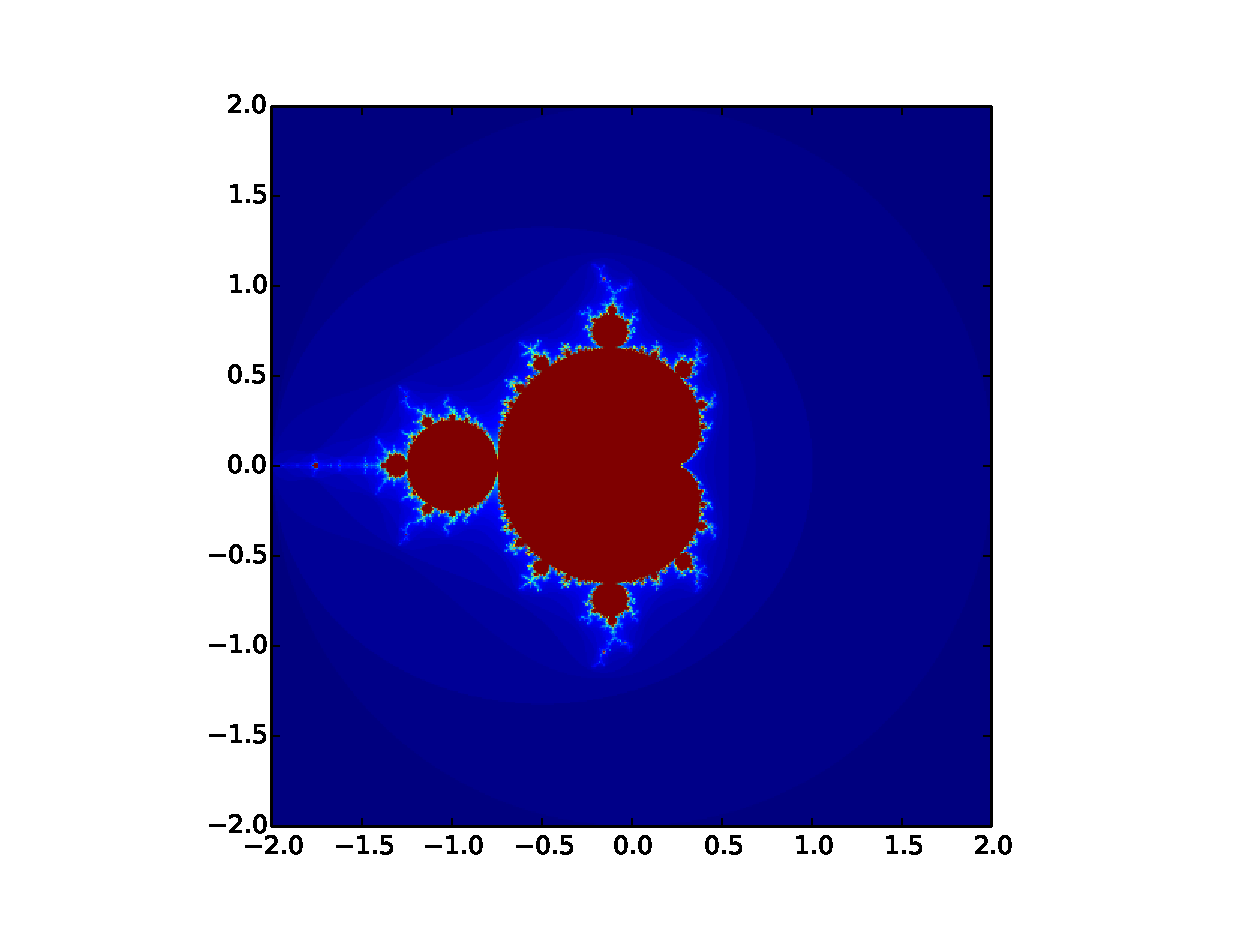
\includegraphics[scale=0.42]{mandel_2.eps}
    \caption{\scriptsize $\nu_{RF}$ vs $B_{H}$ for $^{85}Rb$}
  \end{minipage} \hfill
  \begin{minipage}[t]{0.4\textwidth}
    \centering
    \vspace{0pt}
    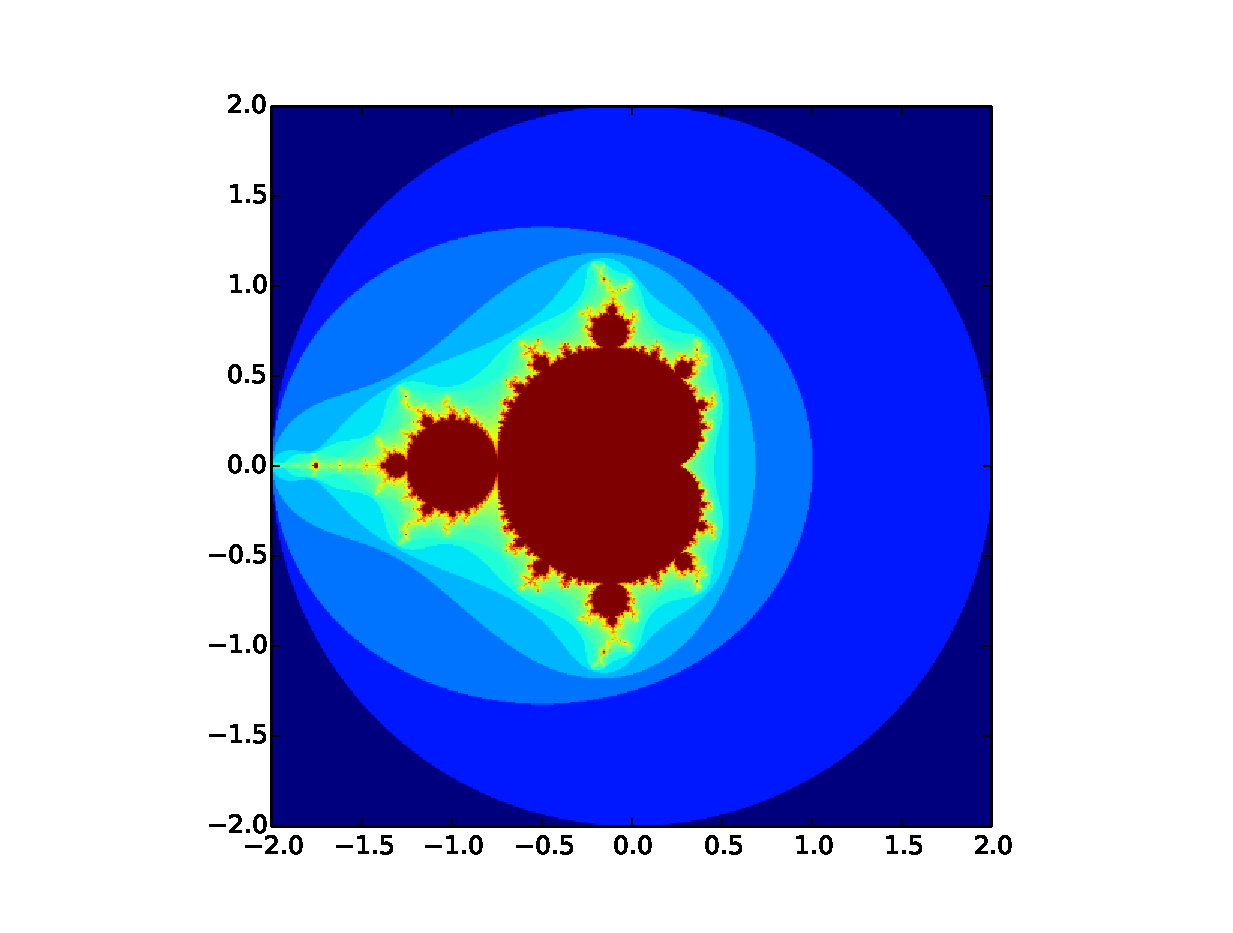
\includegraphics[scale=0.42]{mandel_3.eps}
    \caption{\scriptsize $\nu_{RF}$ vs $B_{H}$ for $^{87}Rb$}
  \end{minipage}
\end{figure}


\section*{Problem 2}
\subsection*{Introduction}
In this problem we wrote our own linear least squares fitting code. 

\subsection*{Methods}
stuff

\subsection*{Results}
plots

\end{document}
